\documentclass[10pt, aspectratio=169]{beamer}

% --- Cấu hình Giao diện & Màu sắc (Theme) ---
\usetheme{Madrid}
\usecolortheme{whale}

% Định nghĩa hệ màu sắc chuyên nghiệp (Deep Blue & Accent Green)
\definecolor{DeepBlue}{RGB}{0, 43, 77}
\definecolor{AccentGreen}{RGB}{17, 202, 160}
\definecolor{LightGray}{RGB}{241, 245, 249}

\setbeamercolor{palette primary}{bg=DeepBlue, fg=white}
\setbeamercolor{palette secondary}{bg=DeepBlue!85, fg=white}
\setbeamercolor{palette tertiary}{bg=DeepBlue!70, fg=white}
\setbeamercolor{titlelike}{parent=palette primary}
\setbeamercolor{structure}{fg=DeepBlue}

% --- Các gói lệnh cần thiết ---
\usepackage[utf8]{inputenc}
\usepackage[vietnamese]{babel} % Hỗ trợ tiếng Việt
\usepackage{amsmath, amssymb}
\usepackage{booktabs} % Cho bảng chuẩn dòng
\usepackage{graphicx}
\usepackage{listings} % Để chèn code hoặc tên tín hiệu mượt mà

% --- Thông tin Đề tài ---
\title[Mô phỏng CPU 8-Core RISC-V]{\textbf{MÔ PHỎNG CPU 8-CORE VỚI KIẾN TRÚC TẬP LỆNH RISC-V}}
\subtitle{Multiple Processing System sử dụng Verilog HDL}
\author[Nhóm Dự Án]{Thực hiện: Nhóm Học Viên}
\institute[Hội Đồng]{Báo Cáo Tiến Độ Dự Án Kiến Trúc Máy Tính}
\date{\today}

\begin{document}

% ==========================================
% SLIDE 1: TRANG TIÊU ĐỀ
% ==========================================
{\setbeamercolor{background canvas}{bg=LightGray}
\begin{frame}[plain]
    \titlepage
\end{frame}}

% ==========================================
% SLIDE 2: MỤC LỤC
% ==========================================
\begin{frame}{Nội Dung Báo Cáo}
    \tableofcontents
\end{frame}

% ==========================================
% SECTION 1: INTRODUCTION
% ==========================================
\section{Giới Thiệu Đề Tài}

% --- SLIDE 1: BỐI CẢNH NGHIÊN CỨU ---
\subsection{Bối cảnh nghiên cứu}
\begin{frame}{Bối Cảnh Nghiên Cứu \& Lý Do Chọn Đề Tài}
    \begin{block}{Giới hạn vật lý của CPU lõi đơn (Single-core)}
        \small
        Việc tăng hiệu năng bộ vi xử lý bằng cách tăng tần số xung nhịp đã đạt tới giới hạn vật lý do hiện tượng quá nhiệt và tiêu hao năng lượng cực lớn (\textbf{Power Wall, Thermal Wall}).
    \end{block}
    
    \vspace{0.15cm}
    
    \begin{block}{Chuyển dịch tất yếu sang Đa lõi (Multi-core)}
        \small
        Tích hợp nhiều lõi xử lý hoạt động độc lập trên cùng một chip để tối ưu hiệu năng tính toán song song.
    \end{block}

    \vspace{0.15cm}

    \begin{alertblock}{Bài toán đặt ra}
        \small
        Giải quyết các vấn đề phức tạp về giao tiếp liên lõi, tranh chấp bus bộ nhớ dùng chung (memory contention) và đồng bộ giữa các luồng xử lý phần cứng.
    \end{alertblock}
\end{frame}

% --- SLIDE 2: CHỦ ĐỀ DỰ ÁN ---
\subsection{Chủ đề của dự án}
\begin{frame}{Chủ Đề Của Dự Án}
    Dự án tập trung nghiên cứu, thiết kế phần cứng ở mức RTL sử dụng ngôn ngữ mô tả phần cứng \textbf{Verilog HDL} để mô phỏng bộ xử lý 8 lõi độc lập:
    
    \vspace{0.2cm}
    \begin{columns}[T]
        \begin{column}{0.48\textwidth}
            \begin{block}{Kiến trúc nhân đơn}
                \small
                Mỗi lõi CPU dựa trên kiến trúc tập lệnh mở \textbf{RISC-V} (\textbf{RV32I subset}) áp dụng kỹ thuật \textbf{pipeline 5 tầng} nhằm tối ưu hóa thông lượng lệnh thực thi.
            \end{block}
        \end{column}
        
        \begin{column}{0.48\textwidth}
            \begin{block}{Kiến trúc đa nhân}
                \small
                Cả 8 nhân CPU kết nối và sử dụng chung một khối bộ nhớ dữ liệu (\textbf{Shared Data Memory}) thông qua một bộ điều khiển Bus và phân xử tập trung.
            \end{block}
        \end{column}
    \end{columns}
\end{frame}

% --- SLIDE 3: MỤC TIÊU THIẾT KẾ ---
\subsection{Mục tiêu thiết kế}
\begin{frame}{Mục Tiêu Thiết Kế}
    Dự án đề ra ba mục tiêu cốt lõi cần đạt được:
    
    \vspace{0.25cm}
    \begin{itemize}
        \item \textbf{Thiết kế lõi đơn:} Thiết kế lõi xử lý RISC-V có pipeline 5 tầng hoàn chỉnh, xử lý xung đột lệnh (data/control hazards) một cách tối ưu bằng Forwarding, Stall và Flush.
        \item \textbf{Thiết kế trục bus đa lõi:} Xây dựng cơ chế phân xử công bằng (Round-Robin Arbiter), đảm bảo cả 8 nhân CPU đều có thể ghi/đọc bộ nhớ dùng chung mà không xảy ra xung đột hay deadlock.
        \item \textbf{Mô phỏng chức năng:} Sử dụng bộ công cụ nguồn mở \textbf{Icarus Verilog} để chạy mô phỏng hệ thống và \textbf{GTKWave} để phân tích giản đồ thời gian (waveform).
    \end{itemize}
\end{frame}
% ==========================================
% SECTION 2: ISA RISC-V 32-bit
% ==========================================
\section{Kiến Trúc Tập Lệnh (ISA)}

\begin{frame}{2.1 Giới Thiệu Tập Lệnh RISC-V (RV32I)}
    \begin{block}{RISC-V là gì?}
        Là một kiến trúc tập lệnh (ISA) mã nguồn mở dựa trên nguyên lý thiết kế máy tính tập lệnh rút gọn (RISC). Cho phép tự do thiết kế, tùy biến và tối ưu hóa phần cứng.
    \end{block}
    
    \vspace{0.2cm}
    \begin{columns}
        \begin{column}{0.65\textwidth}
            \textbf{Giải nghĩa bộ lệnh cơ bản RV32I:}
            \begin{itemize}
                \item \textbf{RV (RISC-V):} Tiêu chuẩn kiến trúc thế hệ thứ 5 từ UC Berkeley.
                \item \textbf{32 (32-bit):} Độ rộng thanh ghi và không gian địa chỉ 32-bit.
                \item \textbf{I (Integer):} Tập lệnh số nguyên cơ bản (gồm 40 lệnh). Đây là tập lệnh bắt buộc phải có cho mọi thiết kế chip RISC-V.
            \end{itemize}
        \end{column}
        \begin{column}{0.32\textwidth}
            \begin{exampleblock}{Mục tiêu lựa chọn}
                Đơn giản hóa thiết kế lõi đơn để tập trung tối ưu bộ điều khiển phân xử (Arbiter) và kết nối đa lõi (8-Core Interconnect).
            \end{exampleblock}
        \end{column}
    \end{columns}
\end{frame}

\begin{frame}{2.2 Đặc Điểm Cốt Lõi của RV32I}
    \begin{columns}
        \begin{column}{0.46\textwidth}
            \textbf{Các đặc trưng kỹ thuật:}
            \begin{itemize}
                \item Không gian địa chỉ và độ dài lệnh cố định \textbf{32-bit}.
                \item Cơ chế \textbf{Load-Store}: Chỉ có lệnh Load/Store mới được truy cập Memory; các phép toán toán học chỉ thực thi trên Tập thanh ghi.
                \item \textbf{32 Thanh ghi đa năng} ($x0 \rightarrow x31$), trong đó $x0$ luôn cố định bằng số $0$.
                \item 6 kiểu định dạng lệnh cơ bản: R, I, S, B, U, J.
            \end{itemize}
        \end{column}
        
        \begin{column}{0.52\textwidth}
            \begin{exampleblock}{Phân loại Tập thanh ghi (Register File)}
                \scriptsize
                \begin{itemize}
                    \item \textcolor{red!80!black}{\textbf{\texttt{x0} (zero):}} Luôn bằng 0 (hằng số phần cứng).
                    \item \textcolor{blue!80!black}{\textbf{\texttt{x1} (ra), \texttt{x2} (sp):}} Địa chỉ trả về \& Con trỏ Stack.
                    \item \textcolor{blue!60!black}{\textbf{\texttt{x3}-\texttt{x4} (gp-tp):}} Con trỏ toàn cục và con trỏ tiểu trình.
                    \item \textcolor{orange!80!black}{\textbf{\texttt{x10}-\texttt{x17} (a0-a7):}} Tham số truyền vào \& Kết quả hàm.
                    \item \textcolor{green!60!black}{\textbf{\texttt{x5}-\texttt{x7}, \texttt{x28}-\texttt{x31} (t0-t6):}} Thanh ghi tạm thời.
                    \item \textcolor{purple!80!black}{\textbf{\texttt{x8}-\texttt{x9}, \texttt{x18}-\texttt{x27} (s0-s11):}} Thanh ghi lưu giữ.
                \end{itemize}
            \end{exampleblock}
        \end{column}
    \end{columns}
\end{frame}

\begin{frame}{2.3 Sáu Kiểu Định Dạng Lệnh Cơ Bản}
    \begin{columns}
        \begin{column}{0.68\textwidth}
            \centering
            \begin{tikzpicture}[
                box/.style={draw, minimum height=0.42cm, font=\scriptsize, align=center, inner sep=0pt},
                f7/.style={box, fill=cyan!15},
                rs2/.style={box, fill=orange!20},
                rs1/.style={box, fill=yellow!20},
                f3/.style={box, fill=green!15},
                rd/.style={box, fill=blue!15},
                op/.style={box, fill=red!15},
                imm/.style={box, fill=purple!15}
            ]
                % Bit indicators
                \node[anchor=south west, font=\tiny\color{gray}] at (0, 0.18) {31};
                \node[anchor=south east, font=\tiny\color{gray}] at (1.8, 0.18) {25};
                \node[anchor=south west, font=\tiny\color{gray}] at (1.8, 0.18) {24};
                \node[anchor=south east, font=\tiny\color{gray}] at (3.1, 0.18) {20};
                \node[anchor=south west, font=\tiny\color{gray}] at (3.1, 0.18) {19};
                \node[anchor=south east, font=\tiny\color{gray}] at (4.4, 0.18) {15};
                \node[anchor=south west, font=\tiny\color{gray}] at (4.4, 0.18) {14};
                \node[anchor=south east, font=\tiny\color{gray}] at (5.4, 0.18) {12};
                \node[anchor=south west, font=\tiny\color{gray}] at (5.4, 0.18) {11};
                \node[anchor=south east, font=\tiny\color{gray}] at (6.7, 0.18) {7};
                \node[anchor=south west, font=\tiny\color{gray}] at (6.7, 0.18) {6};
                \node[anchor=south east, font=\tiny\color{gray}] at (8.5, 0.18) {0};

                % R-type
                \node[f7, minimum width=1.8cm] at (0.9, 0) {funct7};
                \node[rs2, minimum width=1.3cm] at (2.45, 0) {rs2};
                \node[rs1, minimum width=1.3cm] at (3.75, 0) {rs1};
                \node[f3, minimum width=1.0cm] at (4.9, 0) {funct3};
                \node[rd, minimum width=1.3cm] at (6.05, 0) {rd};
                \node[op, minimum width=1.8cm] at (7.6, 0) {opcode};
                \node[anchor=east, font=\scriptsize\bfseries\color{DeepBlue}] at (-0.2, 0) {R-type};

                % I-type
                \node[imm, minimum width=3.1cm] at (1.55, -0.55) {imm[11:0]};
                \node[rs1, minimum width=1.3cm] at (3.75, -0.55) {rs1};
                \node[f3, minimum width=1.0cm] at (4.9, -0.55) {funct3};
                \node[rd, minimum width=1.3cm] at (6.05, -0.55) {rd};
                \node[op, minimum width=1.8cm] at (7.6, -0.55) {opcode};
                \node[anchor=east, font=\scriptsize\bfseries\color{DeepBlue}] at (-0.2, -0.55) {I-type};

                % S-type
                \node[imm, minimum width=1.8cm] at (0.9, -1.1) {imm[11:5]};
                \node[rs2, minimum width=1.3cm] at (2.45, -1.1) {rs2};
                \node[rs1, minimum width=1.3cm] at (3.75, -1.1) {rs1};
                \node[f3, minimum width=1.0cm] at (4.9, -1.1) {funct3};
                \node[imm, minimum width=1.3cm] at (6.05, -1.1) {imm[4:0]};
                \node[op, minimum width=1.8cm] at (7.6, -1.1) {opcode};
                \node[anchor=east, font=\scriptsize\bfseries\color{DeepBlue}] at (-0.2, -1.1) {S-type};

                % B-type
                \node[imm, minimum width=1.8cm] at (0.9, -1.65) {imm[12|10:5]};
                \node[rs2, minimum width=1.3cm] at (2.45, -1.65) {rs2};
                \node[rs1, minimum width=1.3cm] at (3.75, -1.65) {rs1};
                \node[f3, minimum width=1.0cm] at (4.9, -1.65) {funct3};
                \node[imm, minimum width=1.3cm] at (6.05, -1.65) {imm[4:1|11]};
                \node[op, minimum width=1.8cm] at (7.6, -1.65) {opcode};
                \node[anchor=east, font=\scriptsize\bfseries\color{DeepBlue}] at (-0.2, -1.65) {B-type};

                % U-type
                \node[imm, minimum width=5.4cm] at (2.7, -2.2) {imm[31:12]};
                \node[rd, minimum width=1.3cm] at (6.05, -2.2) {rd};
                \node[op, minimum width=1.8cm] at (7.6, -2.2) {opcode};
                \node[anchor=east, font=\scriptsize\bfseries\color{DeepBlue}] at (-0.2, -2.2) {U-type};

                % J-type
                \node[imm, minimum width=5.4cm] at (2.7, -2.75) {imm[20|10:1|11|19:12]};
                \node[rd, minimum width=1.3cm] at (6.05, -2.75) {rd};
                \node[op, minimum width=1.8cm] at (7.6, -2.75) {opcode};
                \node[anchor=east, font=\scriptsize\bfseries\color{DeepBlue}] at (-0.2, -2.75) {J-type};
            \end{tikzpicture}
        \end{column}
        
        \begin{column}{0.31\textwidth}
            \footnotesize
            \begin{block}{Giải thích các trường}
                \begin{itemize}
                    \item \textcolor{red!80!black}{\textbf{opcode}:} Mã lệnh gốc (7 bit).
                    \item \textcolor{blue!80!black}{\textbf{rd}:} Thanh ghi đích.
                    \item \textcolor{green!60!black}{\textbf{funct3/7}:} Mã mở rộng chức năng lệnh.
                    \item \textcolor{orange!80!black}{\textbf{rs1/rs2}:} Các thanh ghi nguồn.
                    \item \textcolor{purple!80!black}{\textbf{imm}:} Giá trị hằng số nạp trực tiếp.
                \end{itemize}
            \end{block}
        \end{column}
    \end{columns}
\end{frame}

\begin{frame}{2.4 Tập Lệnh Hiện Thực Hóa Trong Project}
    \begin{columns}
        \begin{column}{0.5\textwidth}
            \begin{block}{Tập Lệnh Số Nguyên RV32I Subset}
                \textbf{40 lệnh cơ bản được hỗ trợ:}
                \begin{itemize}
                    \item \textbf{Tính toán (ALU):} \texttt{ADD/SUB}, \texttt{SLL/SRL}, \texttt{AND/OR/XOR}, \texttt{SLT} (bao gồm cả dạng hằng số Imm như \texttt{ADDI}, \texttt{ANDI},...).
                    \item \textbf{Bộ nhớ:} \texttt{LW} (Load Word), \texttt{SW} (Store Word).
                    \item \textbf{Điều khiển luồng:} \texttt{BEQ}, \texttt{BNE}, \texttt{BLT}, \texttt{BGE}, \texttt{JAL}, \texttt{JALR}.
                    \item \textbf{Khác:} \texttt{LUI}, \texttt{AUIPC}.
                \end{itemize}
            \end{block}
        \end{column}
        
        \begin{column}{0.48\textwidth}
            \begin{alertblock}{Đồng Bộ Đa Nhân (A-Extension)}
                \textbf{Thiết kế riêng cho hệ thống 8-Core:}
                \begin{itemize}
                    \item \textbf{Độc quyền truy cập:} \texttt{LR.W} (Load-Reserved) và \texttt{SC.W} (Store-Conditional) để xây dựng cấu trúc đồng bộ (Mutex/Semaphore).
                    \item \textbf{Phép toán nguyên tử (AMO):} \texttt{AMOSWAP}, \texttt{AMOADD}, \texttt{AMOAND}, \texttt{AMOOR}, \texttt{AMOXOR}, \texttt{AMOMIN/MAX} trực tiếp trên bộ nhớ dùng chung.
                \end{itemize}
            \end{alertblock}
        \end{column}
    \end{columns}
\end{frame}


% ==========================================
% SECTION 3: DESIGN ARCHITECTURE
% ==========================================
\section{Thiết Kế Hệ Thống (Design)}

\begin{frame}{3. Thiết Kế Hệ Thống: Cấu Trúc Tổng Thể}
    \begin{center}
        \textbf{Sơ đồ phân rã các Module trong mã nguồn Verilog}
    \end{center}
    Hệ thống được chia thành 4 phân vùng chính để quản lý và hiện thực hóa trong mã nguồn:
    \vspace{0.3cm}
    \begin{enumerate}
        \item \textbf{Datapath (Single Core):} Trục xương sống dịch chuyển và biến đổi dữ liệu.
        \item \textbf{Control Unit:} Bộ não điều khiển luồng dữ liệu chạy nhịp nhàng qua Pipeline.
        \item \textbf{Pipeline Hazard Unit:} Khối cứu nguy và xử lý các xung đột phần cứng.
        \item \textbf{Interconnect:} Hệ thống trục Bus kết nối, phân xử quyền hạn giữa 8 lõi CPU.
    \end{enumerate}
\end{frame}


\begin{frame}{Phân bố phần cứng trên 5 tầng Pipeline}
    Đường truyền dữ liệu (Datapath) ánh xạ trực tiếp các module Verilog vào từng giai đoạn xử lý:
    \vspace{0.3cm}
    
    \centering
    \begin{tikzpicture}[
        stage/.style={draw=DeepBlue, fill=DeepBlue!6, minimum width=1.8cm, minimum height=1.2cm, rounded corners=4pt, line width=1.2pt, font=\scriptsize, text width=1.75cm, align=center},
        reg/.style={draw=AccentGreen!80!black, fill=AccentGreen!12, minimum width=0.4cm, minimum height=1.8cm, rounded corners=1.5pt, line width=1.2pt, font=\tiny\bfseries\color{DeepBlue!90!black}, align=center},
        arrow/.style={->, >=stealth, line width=1.5pt, DeepBlue!85}
    ]
        % Stages & Registers
        \node[stage] (if) at (0.9, 0) {\textbf{Fetch (IF)}\\[0.05cm]\tiny\color{black!70}\texttt{pc\_logic}\\[0.02cm]\tiny\color{black!70}\texttt{instr\_mem}};
        \node[reg] (ifid) at (2.3, 0) {\makebox[0pt][c]{\rotatebox{90}{IF/ID}}};
        
        \node[stage] (id) at (3.7, 0) {\textbf{Decode (ID)}\\[0.05cm]\tiny\color{black!70}\texttt{control\_unit}\\[0.02cm]\tiny\color{black!70}\texttt{reg\_file}};
        \node[reg] (idex) at (5.1, 0) {\makebox[0pt][c]{\rotatebox{90}{ID/EX}}};
        
        \node[stage] (ex) at (6.5, 0) {\textbf{Execute (EX)}\\[0.05cm]\tiny\color{black!70}\texttt{alu}};
        \node[reg] (exmem) at (7.9, 0) {\makebox[0pt][c]{\rotatebox{90}{EX/MEM}}};
        
        \node[stage] (mem) at (9.3, 0) {\textbf{Memory (MEM)}\\[0.05cm]\tiny\color{black!70}Liên kết\\[0.02cm]\tiny\color{black!70}\texttt{data\_mem}};
        \node[reg] (memwb) at (10.7, 0) {\makebox[0pt][c]{\rotatebox{90}{MEM/WB}}};
        
        \node[stage] (wb) at (12.1, 0) {\textbf{Writeback (WB)}\\[0.05cm]\tiny\color{black!70}Ghi tập\\[0.02cm]\tiny\color{black!70}thanh ghi};
        
        % Clock triangles at the bottom of pipeline registers
        \draw[line width=1.2pt, AccentGreen!80!black] (2.2, -0.9) -- (2.3, -0.78) -- (2.4, -0.9);
        \draw[line width=1.2pt, AccentGreen!80!black] (5.0, -0.9) -- (5.1, -0.78) -- (5.2, -0.9);
        \draw[line width=1.2pt, AccentGreen!80!black] (7.8, -0.9) -- (7.9, -0.78) -- (8.0, -0.9);
        \draw[line width=1.2pt, AccentGreen!80!black] (10.6, -0.9) -- (10.7, -0.78) -- (10.8, -0.9);
        
        % Connections
        \draw[arrow] (if.east) -- (ifid.west);
        \draw[arrow] (ifid.east) -- (id.west);
        \draw[arrow] (id.east) -- (idex.west);
        \draw[arrow] (idex.east) -- (ex.west);
        \draw[arrow] (ex.east) -- (exmem.west);
        \draw[arrow] (exmem.east) -- (mem.west);
        \draw[arrow] (mem.east) -- (memwb.west);
        \draw[arrow] (memwb.east) -- (wb.west);
    \end{tikzpicture}
    
    \vspace{0.3cm}
    \begin{block}{Nguyên lý hoạt động của Đường dữ liệu}
        \scriptsize
        \begin{itemize}
            \item \textbf{Khối logic chức năng} (\texttt{pc\_logic}, \texttt{reg\_file}, \texttt{alu},...) thực hiện nhiệm vụ xử lý trong từng tầng riêng biệt.
            \item \textbf{Thanh ghi đệm Pipeline} (\texttt{IF/ID}, \texttt{ID/EX},...) đóng vai trò chốt dữ liệu giữa các sườn clock, giữ cho lệnh ở các tầng không bị trộn lẫn khi thực thi song song.
        \end{itemize}
    \end{block}
\end{frame}

\subsection{Các khối xử lý logic chức năng}
\subsubsection{Bộ nhớ lệnh (Instruction Memory)}
\begin{frame}[fragile]{Bộ nhớ lệnh (\texttt{instr\_mem.v})}
    \begin{columns}
        \begin{column}{0.48\textwidth}
            \centering
            \textbf{Sơ đồ khối chức năng}
            \vspace{0.3cm}
            
            \begin{tikzpicture}[
                block/.style={draw, thick, fill=blue!10, draw=DeepBlue, minimum width=3.2cm, minimum height=1.8cm, rounded corners, font=\scriptsize\bfseries, align=center},
                bus/.style={->, >=stealth, double, double distance=1.5pt, thick, DeepBlue}
            ]
                % Main Memory Block
                \node[block] (mem) at (0, 0) {Instruction Memory\\[0.15cm]\tiny (\texttt{instr\_mem.v})\\[0.2cm]\scriptsize Mảng nhớ: 256 $\times$ 32-bit};
                
                % Inputs
                \draw[bus] (-2.6, 0) -- node[above=0.05cm, font=\tiny\bfseries] {addr[31:0]} (mem.west);
                
                % Outputs
                \draw[bus] (mem.east) -- node[above=0.05cm, font=\tiny\bfseries] {instruction[31:0]} (2.6, 0);
            \end{tikzpicture}
        \end{column}
        
        \begin{column}{0.48\textwidth}
            \begin{block}{Mã nguồn Verilog đầy đủ}
                \begin{lstlisting}[language=Verilog, basicstyle=\tiny\ttfamily, keywordstyle=\color{blue}, commentstyle=\color{gray}]
module instr_mem #(
    parameter INIT_FILE = "program.hex",
    parameter PROGRAM_WORDS = 256
)(
    input  wire [31:0] addr,
    output wire [31:0] instruction
);
    reg [31:0] mem [0:255];
    wire [7:0] word_addr = addr[9:2];

    assign instruction = mem[word_addr];

    integer i;
    initial begin
        // Khoi tao NOP truoc khi nap
        for (i = 0; i < 256; i = i + 1)
            mem[i] = 32'h0000_0013;
        $readmemh(INIT_FILE, mem, 0, PROGRAM_WORDS - 1);
    end
endmodule
                \end{lstlisting}
            \end{block}
        \end{column}
    \end{columns}
\end{frame}
\subsubsection{Khối PC Logic}
\begin{frame}[fragile]{PC Logic: Sơ đồ \& Nguyên lý hoạt động}
    \begin{columns}
        \begin{column}{0.48\textwidth}
            \centering
            \textbf{Sơ đồ khối chức năng}
            \vspace{0.2cm}
            
            \begin{tikzpicture}[
                block/.style={draw, thick, fill=blue!10, draw=DeepBlue, minimum width=3.0cm, minimum height=2.8cm, rounded corners, font=\scriptsize\bfseries, align=center},
                bus/.style={->, >=stealth, double, double distance=1.5pt, thick, DeepBlue},
                wire/.style={->, >=stealth, thick, DeepBlue}
            ]
                % Main Block
                \node[block] (pc_block) at (0, 0) {PC Logic\\[0.15cm]\tiny (\texttt{pc\_logic.v})};
                
                % Inputs (Left side)
                \draw[wire] (-2.2, 1.05) -- node[above, font=\tiny\bfseries] {clk} ([yshift=1.05cm]pc_block.west);
                \draw[wire] (-2.2, 0.70) -- node[above, font=\tiny\bfseries] {reset} ([yshift=0.70cm]pc_block.west);
                \draw[wire] (-2.2, 0.35) -- node[above, font=\tiny\bfseries] {stall} ([yshift=0.35cm]pc_block.west);
                
                \draw[wire] (-2.2, -0.15) -- node[above, font=\tiny\bfseries] {branch\_taken} ([yshift=-0.15cm]pc_block.west);
                \draw[bus] (-2.2, -0.50) -- node[above=0.02cm, font=\tiny\bfseries] {branch\_target} ([yshift=-0.50cm]pc_block.west);
                
                \draw[wire] (-2.2, -0.85) -- node[above, font=\tiny\bfseries] {jump} ([yshift=-0.85cm]pc_block.west);
                \draw[bus] (-2.2, -1.20) -- node[above=0.02cm, font=\tiny\bfseries] {jump\_target} ([yshift=-1.20cm]pc_block.west);
                
                % Outputs (Right side)
                \draw[bus] (pc_block.east) -- node[above=0.05cm, font=\tiny\bfseries] {pc[31:0]} (2.2, 0);
            \end{tikzpicture}
        \end{column}
        
        \begin{column}{0.48\textwidth}
            \begin{block}{Nguyên lý cập nhật địa chỉ PC}
                \scriptsize
                Quy trình cập nhật PC theo mức độ ưu tiên giảm dần:
                \begin{enumerate}
                    \item \textbf{Reset:} Đưa địa chỉ PC về 0 khi bắt đầu.
                    \item \textbf{Stall:} Đóng băng PC (giữ nguyên giá trị cũ) khi gặp xung đột dữ liệu hoặc tài nguyên.
                    \item \textbf{Jump:} Nhập địa chỉ nhảy không điều kiện (`jump\_target`) từ các lệnh `JAL`, `JALR`.
                    \item \textbf{Branch:} Nhập địa chỉ rẽ nhánh (`branch\_target`) khi điều kiện rẽ nhánh thỏa mãn (\texttt{branch\_taken} = 1).
                \end{enumerate}
            \end{block}
        \end{column}
    \end{columns}
\end{frame}

\begin{frame}[fragile]{PC Logic: Hiện thực mã nguồn Verilog}
    \begin{columns}[t]
        \begin{column}{0.46\textwidth}
            \begin{block}{Khai báo Module \& Ports}
                \begin{lstlisting}[language=Verilog, basicstyle=\fontsize{6.5pt}{8.0pt}\selectfont\ttfamily, keywordstyle=\color{blue}, commentstyle=\color{gray}]
module pc_logic (
    input  wire        clk,
    input  wire        reset,
    input  wire        stall,

    input  wire        branch_taken,
    input  wire [31:0] branch_target,

    input  wire        jump,
    input  wire [31:0] jump_target,

    output reg  [31:0] pc
);
                \end{lstlisting}
            \end{block}
        \end{column}
        
        \begin{column}{0.50\textwidth}
            \begin{block}{Khối Logic Cập Nhật PC}
                \begin{lstlisting}[language=Verilog, basicstyle=\fontsize{6.5pt}{8.0pt}\selectfont\ttfamily, keywordstyle=\color{blue}, commentstyle=\color{gray}]
    always @(posedge clk or posedge reset) begin
        if (reset) begin
            pc <= 32'd0;
        end
        else if (stall) begin
            pc <= pc;
        end
        else if (jump) begin
            pc <= jump_target;
        end
        else if (branch_taken) begin
            pc <= branch_target;
        end
        else begin
            pc <= pc + 32'd4;
        end
    end

endmodule
                \end{lstlisting}
            \end{block}
        \end{column}
    \end{columns}
\end{frame}

\begin{frame}[fragile]{PC Logic: Thiết lập môi trường Testbench}
    \begin{columns}[t]
        \begin{column}{0.46\textwidth}
            \begin{block}{Khai báo Tín hiệu \& Mạch nạp}
                \begin{lstlisting}[language=Verilog, basicstyle=\fontsize{6.5pt}{8.0pt}\selectfont\ttfamily, keywordstyle=\color{blue}, commentstyle=\color{gray}]
`timescale 1ns/1ps

module pc_logic_tb;

    reg clk;
    reg reset;
    reg stall;

    reg branch_taken;
    reg [31:0] branch_target;

    reg jump;
    reg [31:0] jump_target;

    wire [31:0] pc;
                \end{lstlisting}
            \end{block}
        \end{column}
        
        \begin{column}{0.50\textwidth}
            \begin{block}{Khởi tạo UUT \& Bộ tạo Xung nhịp}
                \begin{lstlisting}[language=Verilog, basicstyle=\fontsize{6.5pt}{7.5pt}\selectfont\ttfamily, keywordstyle=\color{blue}, commentstyle=\color{gray}]
    pc_logic uut (
        .clk(clk),
        .reset(reset),
        .stall(stall),
        .branch_taken(branch_taken),
        .branch_target(branch_target),
        .jump(jump),
        .jump_target(jump_target),
        .pc(pc)
    );

    always #5 clk = ~clk;
                \end{lstlisting}
            \end{block}
        \end{column}
    \end{columns}
\end{frame}

\begin{frame}[fragile]{PC Logic: Kịch bản kiểm thử}
    \begin{columns}[t]
        \begin{column}{0.48\textwidth}
            \begin{block}{Kịch bản kích thích chính}
                \begin{lstlisting}[language=Verilog, basicstyle=\fontsize{6.5pt}{8.0pt}\selectfont\ttfamily, keywordstyle=\color{blue}, commentstyle=\color{gray}]
    initial begin
        clk = 0; reset = 1; stall = 0;
        branch_taken = 0; branch_target = 0;
        jump = 0; jump_target = 0;
        #10 reset = 0;
        #20; // Normal PC increment
        stall = 1; #10; stall = 0; // Stall
        branch_taken = 1; branch_target = 100;
        #10; branch_taken = 0; // Branch
        jump = 1; jump_target = 200;
        #10; jump = 0; // Jump
        #20; $finish;
    end
                \end{lstlisting}
            \end{block}
        \end{column}
        
        \begin{column}{0.48\textwidth}
            \begin{block}{Giám sát tín hiệu \& Lưu dạng sóng}
                \begin{lstlisting}[language=Verilog, basicstyle=\fontsize{6.5pt}{8.0pt}\selectfont\ttfamily, keywordstyle=\color{blue}, commentstyle=\color{gray}]
    initial begin
        $monitor(
            "t=%0t pc=%0d s=%b b=%b j=%b",
            $time, pc, stall, branch_taken, jump
        );
    end

    initial begin
        $dumpfile("pc_logic_tb.vcd");
        $dumpvars(0, pc_logic_tb);
    end

endmodule
                \end{lstlisting}
            \end{block}
        \end{column}
    \end{columns}
\end{frame}
\begin{frame}[fragile]{PC Logic: Kết Quả Mô Phỏng Console}
    \begin{columns}
        \begin{column}{0.55\textwidth}
            \begin{block}{Console Output (\$monitor)}
                \begin{lstlisting}[basicstyle=\fontsize{7.5pt}{9.0pt}\selectfont\ttfamily, numbers=none]
Time=0 | PC=         0 | stall=0 | branch=0 | jump=0
Time=15000 | PC=         4 | stall=0 | branch=0 | jump=0
Time=25000 | PC=         8 | stall=0 | branch=0 | jump=0
Time=30000 | PC=         8 | stall=1 | branch=0 | jump=0
Time=40000 | PC=         8 | stall=0 | branch=1 | jump=0
Time=45000 | PC=       100 | stall=0 | branch=1 | jump=0
Time=50000 | PC=       100 | stall=0 | branch=0 | jump=1
Time=55000 | PC=       200 | stall=0 | branch=0 | jump=1
Time=60000 | PC=       200 | stall=0 | branch=0 | jump=0
Time=65000 | PC=       204 | stall=0 | branch=0 | jump=0
Time=75000 | PC=       208 | stall=0 | branch=0 | jump=0
tb/pc_logic_tb.v:63: $finish called at 80000 (1ps)
                \end{lstlisting}
            \end{block}
        \end{column}
        
        \begin{column}{0.41\textwidth}
            \begin{block}{Phân tích kịch bản kiểm thử}
                \scriptsize
                \begin{itemize}
                    \item \textbf{0ns -- 30ns (Tăng tuần tự):} PC tăng tuần tự +4 sau mỗi chu kỳ clock (0 $\rightarrow$ 4 $\rightarrow$ 8).
                    \item \textbf{30ns -- 40ns (Đóng băng):} Tín hiệu \texttt{stall=1}, PC giữ nguyên giá trị bằng 8.
                    \item \textbf{40ns -- 50ns (Rẽ nhánh):} Tín hiệu \texttt{branch\_taken=1}, PC cập nhật địa chỉ nhánh bằng 100.
                    \item \textbf{50ns -- 60ns (Lệnh nhảy):} Tín hiệu \texttt{jump=1}, PC cập nhật địa chỉ nhảy bằng 200.
                \end{itemize}
            \end{block}
        \end{column}
    \end{columns}
\end{frame}

\begin{frame}{PC Logic: Giản Đồ Sóng Mô Phỏng (GTKWave)}
    \begin{block}{Giản đồ sóng chi tiết}
        \centering
        \vspace{0.05cm}
        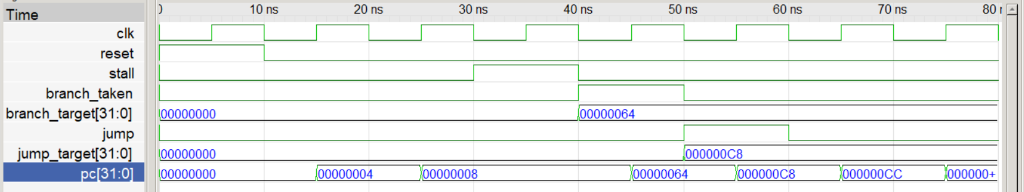
\includegraphics[width=0.98\textwidth]{design/test/pc_test.png}
        \vspace{0.05cm}
    \end{block}
    \vspace{0.1cm}
    \begin{block}{Nhận xét kết quả trên dạng sóng}
        \scriptsize
        \begin{itemize}
            \item \textbf{Thời điểm 30ns (Stall):} Khi \texttt{stall} lên 1, giá trị PC được chốt giữ nguyên ở mức 8 tại sườn lên clock tiếp theo.
            \item \textbf{Thời điểm 40ns (Branch):} Địa chỉ rẽ nhánh \texttt{branch\_target} = \texttt{0x00000064} (100) được nạp thành công vào PC.
            \item \textbf{Thời điểm 50ns (Jump):} Địa chỉ nhảy \texttt{jump\_target} = \texttt{0x000000C8} (200) được cập nhật thành công vào PC.
        \end{itemize}
    \end{block}
\end{frame}
\subsubsection{Khối Tập thanh ghi (Register File)}
\begin{frame}[fragile]{Khối Tập Thanh Ghi (\texttt{reg\_file.v})}
    \begin{columns}
        \begin{column}{0.46\textwidth}
            \centering
            \textbf{Sơ đồ khối chức năng}
            \vspace{0.2cm}
            
            \begin{tikzpicture}[
                block/.style={draw, thick, fill=blue!10, draw=DeepBlue, minimum width=2.8cm, minimum height=2.6cm, rounded corners, font=\scriptsize\bfseries, align=center},
                bus/.style={->, >=stealth, double, double distance=1.5pt, thick, DeepBlue},
                wire/.style={->, >=stealth, thick, DeepBlue}
            ]
                % Main Block
                \node[block] (rf) at (0, 0) {Register File\\[0.1cm]\tiny (\texttt{reg\_file.v})};
                
                % Inputs (Left side)
                \draw[wire] (-2.0, 0.9) -- node[above, font=\tiny\bfseries] {clk} ([yshift=0.9cm]rf.west);
                \draw[bus] (-2.0, 0.4) -- node[above=0.01cm, font=\tiny\bfseries] {rs1\_addr} ([yshift=0.4cm]rf.west);
                \draw[bus] (-2.0, 0.0) -- node[above=0.01cm, font=\tiny\bfseries] {rs2\_addr} ([yshift=0.0cm]rf.west);
                \draw[bus] (-2.0, -0.4) -- node[above=0.01cm, font=\tiny\bfseries] {rd\_addr} ([yshift=-0.4cm]rf.west);
                \draw[bus] (-2.0, -0.9) -- node[above=0.01cm, font=\tiny\bfseries] {wdata} ([yshift=-0.9cm]rf.west);
                
                % Control Input (Top side)
                \draw[wire] (0, 1.7) -- node[right, font=\tiny\bfseries] {reg\_write} (rf.north);
                
                % Outputs (Right side)
                \draw[bus] ([yshift=0.4cm]rf.east) -- node[above=0.01cm, font=\tiny\bfseries] {rs1\_data} (2.0, 0.4);
                \draw[bus] ([yshift=-0.4cm]rf.east) -- node[above=0.01cm, font=\tiny\bfseries] {rs2\_data} (2.0, -0.4);
            \end{tikzpicture}
            
            \vspace{0.15cm}
            \scriptsize
            \begin{block}{Nguyên lý hoạt động}
                \begin{itemize}
                    \item \textbf{Quy mô:} 32 thanh ghi 32-bit (x0 cứng về 0).
                    \item \textbf{Đọc bất đồng bộ:} rs1\_data, rs2\_data.
                    \item \textbf{Ghi đồng bộ:} rd khi reg\_write=1.
                    \item \textbf{Cầu bypass:} Tránh trễ 1 chu kỳ khi đọc-ghi cùng thanh ghi.
                \end{itemize}
            \end{block}
        \end{column}
        
        \begin{column}{0.52\textwidth}
            \begin{block}{Mã nguồn Verilog tập thanh ghi}
                \begin{lstlisting}[language=Verilog, basicstyle=\fontsize{6.0pt}{6.8pt}\selectfont\ttfamily, keywordstyle=\color{blue}, commentstyle=\color{gray}]
module reg_file (
    input  wire        clk, reset,
    input  wire [4:0]  rs1_addr, rs2_addr, rd_addr,
    input  wire [31:0] write_data,
    input  wire        reg_write,
    output wire [31:0] rs1_data, rs2_data
);
    reg [31:0] registers [0:31];

    assign rs1_data = (rs1_addr == 5'd0) ? 32'd0 :
                      (reg_write && (rd_addr == rs1_addr)) 
                      ? write_data : registers[rs1_addr];
    assign rs2_data = (rs2_addr == 5'd0) ? 32'd0 :
                      (reg_write && (rd_addr == rs2_addr)) 
                      ? write_data : registers[rs2_addr];

    integer i;
    always @(posedge clk or posedge reset) begin
        if (reset) begin
            for (i = 0; i < 32; i = i + 1)
                registers[i] <= 32'd0;
        end else if (reg_write && (rd_addr != 5'd0)) begin
            registers[rd_addr] <= write_data;
        end
    end
endmodule
                \end{lstlisting}
            \end{block}
        \end{column}
    \end{columns}
\end{frame}

\subsubsection{Khối Tính toán Số học \& Logic (ALU)}
\begin{frame}[fragile]{Khối Tính Toán Số Học \& Logic (\texttt{alu.v})}
    \begin{columns}
        \begin{column}{0.46\textwidth}
            \centering
            \textbf{Sơ đồ khối chức năng}
            \vspace{0.2cm}
            
            \begin{tikzpicture}[
                alu/.style={draw, thick, fill=blue!10, draw=DeepBlue, minimum width=2.4cm, minimum height=1.6cm, font=\scriptsize\bfseries, align=center},
                bus/.style={->, >=stealth, double, double distance=1.5pt, thick, DeepBlue},
                wire/.style={->, >=stealth, thick, DeepBlue}
            ]
                % Main ALU Block
                \node[alu] (alu_block) at (0, 0) {ALU\\[0.15cm]\tiny (\texttt{alu.v})};
                
                % Inputs
                \draw[bus] (-2.2, 0.4) -- node[above=0.01cm, font=\tiny\bfseries] {a[31:0]} ([yshift=0.4cm]alu_block.west);
                \draw[bus] (-2.2, -0.4) -- node[above=0.01cm, font=\tiny\bfseries] {b[31:0]} ([yshift=-0.4cm]alu_block.west);
                \draw[bus] (0, 1.4) -- node[right, font=\tiny\bfseries] {alu\_control[3:0]} (alu_block.north);
                
                % Outputs
                \draw[bus] ([yshift=0.3cm]alu_block.east) -- node[above=0.01cm, font=\tiny\bfseries] {result[31:0]} (2.2, 0.3);
                \draw[wire] ([yshift=-0.3cm]alu_block.east) -- node[above=0.01cm, font=\tiny\bfseries] {zero} (2.2, -0.3);
            \end{tikzpicture}
            
            \vspace{0.2cm}
            \scriptsize
            \begin{block}{Đặc tả hoạt động}
                \begin{itemize}
                    \item \textbf{Phép toán số học:} ADD (cộng), SUB (trừ), so sánh có dấu SLT.
                    \item \textbf{Phép toán logic:} AND, OR, XOR và dịch chuyển bit logic (SLL, SRL).
                    \item \textbf{Cờ Zero:} Tín hiệu ra 1-bit, tích cực mức cao khi kết quả toán học bằng 0 (dùng cho lệnh rẽ nhánh).
                \end{itemize}
            \end{block}
        \end{column}
        
        \begin{column}{0.52\textwidth}
            \begin{block}{Hiện thực khối Case ALU}
                \begin{lstlisting}[language=Verilog, basicstyle=\fontsize{6.0pt}{7.2pt}\selectfont\ttfamily, keywordstyle=\color{blue}, commentstyle=\color{gray}]
always @(*) begin
    case (alu_control)
        4'b0010: result = a + b; // ADD
        4'b0110: result = a - b; // SUB
        4'b0000: result = a & b; // AND
        4'b0001: result = a | b; // OR
        4'b0100: result = a ^ b; // XOR
        4'b0011: result = a << b[4:0]; // SLL
        4'b0101: result = a >> b[4:0]; // SRL
        4'b0111: result = ($signed(a) < $signed(b)) 
                          ? 32'd1 : 32'd0; // SLT
        default: result = 32'b0;
    endcase
end

// Co bao Zero
assign zero = (result == 32'b0);
                \end{lstlisting}
            \end{block}
        \end{column}
    \end{columns}
\end{frame}

\begin{frame}[fragile]{ALU: Kịch bản kiểm thử (Testbench)}
    \begin{columns}[t]
        \begin{column}{0.48\textwidth}
            \begin{block}{DUT \& Khai báo tín hiệu}
                \begin{lstlisting}[language=Verilog, basicstyle=\fontsize{6.0pt}{7.0pt}\selectfont\ttfamily, keywordstyle=\color{blue}, commentstyle=\color{gray}]
module alu_tb();
    reg  [31:0] a, b;
    reg  [3:0]  alu_control;
    wire [31:0] result;
    wire        zero;

    // Khoi tao Device Under Test (DUT)
    alu dut (
        .a(a), .b(b),
        .alu_control(alu_control),
        .result(result), .zero(zero)
    );

    localparam AND  = 4'b0000;
    localparam OR   = 4'b0001;
    localparam ADD  = 4'b0010;
    localparam SLL  = 4'b0011;
    localparam XOR  = 4'b0100;
    localparam SRL  = 4'b0101;
    localparam SUB  = 4'b0110;
    localparam SLT  = 4'b0111;
                \end{lstlisting}
            \end{block}
        \end{column}
        
        \begin{column}{0.48\textwidth}
            \begin{block}{Kịch bản kích thích chính}
                \begin{lstlisting}[language=Verilog, basicstyle=\fontsize{6.0pt}{7.0pt}\selectfont\ttfamily, keywordstyle=\color{blue}, commentstyle=\color{gray}]
    initial begin
        $dumpfile("tb/alu_tb.vcd");
        $dumpvars(0, alu_tb);
        // Cases: ADD, SUB, AND, SLT (pos/neg)
        a = 10; b = 20; alu_control = ADD; #10;
        a = 50; b = 50; alu_control = SUB; #10;
        a = 32'hAAAA_AAAA; b = 32'h5555_5555; 
        alu_control = AND; #10;
        a = 15; b = 25; alu_control = SLT; #10;
        a = -10; b = 5; alu_control = SLT; #10;
        // Cases: OR, XOR, SLL, SRL
        a = 32'hF0F0_FFFF; b = 32'h0F0F_0000; 
        alu_control = OR; #10;
        a = 32'hF0F0_FFFF; b = 32'hFFFF_0000; 
        alu_control = XOR; #10;
        a = 32'h0000_000F; b = 4; alu_control = SLL; #10;
        a = 32'hF000_0000; b = 4; alu_control = SRL; #10;
        $finish;
    end
                \end{lstlisting}
            \end{block}
        \end{column}
    \end{columns}
\end{frame}

\begin{frame}[fragile]{ALU: Kết quả mô phỏng Console}
    Mô phỏng thực thi chính xác toàn bộ 9 kịch bản kiểm thử trên Console:
    \vspace{0.1cm}
    
    \begin{block}{Kết quả xuất ra màn hình (Console Output)}
        \begin{lstlisting}[basicstyle=\fontsize{5.5pt}{6.5pt}\selectfont\ttfamily]
Time |     A (Hex) [Dec]     |     B (Hex) [Dec]     | Control |   Result [Dec]    | Zero
-----|-----------------------|-----------------------|---------|-------------------|-----
  10 | 0x0000000a (  10)     | 0x00000014 (  20)     |   ADD   | 0x0000001e (  30) |  0
  20 | 0x00000032 (  50)     | 0x00000032 (  50)     |   SUB   | 0x00000000 (   0) |  1
  30 | 0xaaaaaaaa (-1.43G)   | 0x55555555 ( 1.43G)   |   AND   | 0x00000000 (   0) |  1
  40 | 0x0000000f (  15)     | 0x00000019 (  25)     |   SLT   | 0x00000001 (   1) |  0
  50 | 0xfffffff6 ( -10)     | 0x00000005 (   5)     |   SLT   | 0x00000001 (   1) |  0
  60 | 0xf0f0ffff (-252M)    | 0x0f0f0000 ( 252M)    |   OR    | 0xffffffff (  -1) |  0
  70 | 0xf0f0ffff (-252M)    | 0xffff0000 ( -65K)    |   XOR   | 0x0f0fffff ( 252M)|  0
  80 | 0x0000000f (  15)     | 0x00000004 (   4)     |   SLL   | 0x000000f0 ( 240) |  0
  90 | 0xf0000000 (-268M)    | 0x00000004 (   4)     |   SRL   | 0x0f000000 ( 251M)|  0
-----|-----------------------|-----------------------|---------|-------------------|-----
Kiem tra ket thuc.
        \end{lstlisting}
    \end{block}
    
    \vspace{-0.05cm}
    \scriptsize
    \textbf{Nhận xét kết quả:}
    \begin{itemize}
        \item \textbf{Phép toán số học \& logic:} Cộng (`ADD`), trừ (`SUB`), `AND`, `OR`, `XOR` cho kết quả chính xác 100\%.
        \item \textbf{So sánh có dấu SLT:} Kiểm chứng đúng cho cả số dương và số âm ($-10 < 5$ ra kết quả bằng `1`).
        \item \textbf{Dịch chuyển bit SLL/SRL:} Dịch chuyển đúng số bit được yêu cầu (ví dụ: dịch trái `0xF` đi 4 bit ra `0xF0`).
        \item \textbf{Cờ Zero:} Tự động phản hồi lên `1` khi kết quả tính toán bằng 0 (như ở phép `SUB` và `AND`).
    \end{itemize}
\end{frame}

\begin{frame}{ALU: Giản Đồ Sóng Mô Phỏng (GTKWave)}
    \begin{block}{Giản đồ sóng chi tiết thu được từ bộ mô phỏng}
        \centering
        \vspace{0.05cm}
        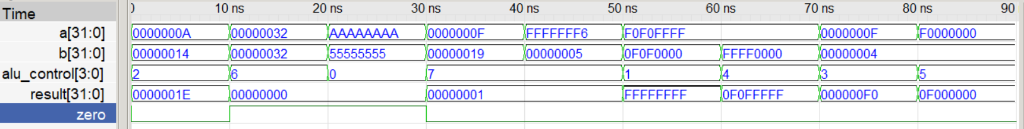
\includegraphics[width=0.95\textwidth]{design/test/alu_test.png}
        \vspace{0.05cm}
    \end{block}
    \vspace{0.15cm}
    \begin{columns}[t]
        \begin{column}{0.48\textwidth}
            \small\textbf{\color{DeepBlue}$\bullet$ Tín hiệu ngõ vào (Inputs)}
            \vspace{0.05cm}
            \scriptsize
            \begin{itemize}
                \item \texttt{a[31:0]}, \texttt{b[31:0]}: Toán hạng ngõ vào (dạng Hex).
                \item \texttt{alu\_control[3:0]}: Mã lệnh điều khiển (\texttt{2}=ADD, \texttt{6}=SUB, \texttt{0}=AND, \texttt{7}=SLT, \texttt{1}=OR, \texttt{4}=XOR, \texttt{3}=SLL, \texttt{5}=SRL).
            \end{itemize}
        \end{column}
        
        \begin{column}{0.48\textwidth}
            \small\textbf{\color{DeepBlue}$\bullet$ Tín hiệu ngõ ra (Outputs)}
            \vspace{0.05cm}
            \scriptsize
            \begin{itemize}
                \item \texttt{result[31:0]}: Kết quả tính toán (dạng Hex).
                \item \texttt{zero}: Cờ báo bằng không, mức cao (\texttt{1}) khi \texttt{result} = 0.
            \end{itemize}
        \end{column}
    \end{columns}
\end{frame}


\subsubsection{Bộ nhớ dữ liệu (Data Memory)}
\begin{frame}[fragile]{Bộ Nhớ Dữ Liệu Dùng Chung (\texttt{data\_mem.v})}
    \begin{columns}
        \begin{column}{0.46\textwidth}
            \centering
            \textbf{Sơ đồ khối chức năng}
            \vspace{0.2cm}
            
            \begin{tikzpicture}[
                block/.style={draw, thick, fill=blue!10, draw=DeepBlue, minimum width=3.0cm, minimum height=2.4cm, rounded corners, font=\scriptsize\bfseries, align=center},
                bus/.style={->, >=stealth, double, double distance=1.5pt, thick, DeepBlue},
                ctrl/.style={->, >=stealth, thick, red!70!black}
            ]
                % Main Block
                \node[block] (mem) at (0, 0) {Shared RAM 4KB\\[0.1cm]\tiny (\texttt{data\_mem.v})};
                
                % Control Inputs (Left side - Red lines)
                \draw[ctrl] (-2.2, 0.9) -- node[above, font=\tiny\bfseries] {clk} ([yshift=0.9cm]mem.west);
                \draw[ctrl] (-2.2, 0.6) -- node[above, font=\tiny\bfseries] {reset} ([yshift=0.6cm]mem.west);
                \draw[ctrl] (-2.2, 0.3) -- node[above, font=\tiny\bfseries] {we} ([yshift=0.3cm]mem.west);
                \draw[ctrl] (-2.2, 0.0) -- node[above, font=\tiny\bfseries] {re} ([yshift=0.0cm]mem.west);
                
                % Data/Address Inputs (Left side - Double Blue lines)
                \draw[bus] (-2.2, -0.4) -- node[above=0.01cm, font=\tiny\bfseries] {addr[31:0]} ([yshift=-0.4cm]mem.west);
                \draw[bus] (-2.2, -0.8) -- node[above=0.01cm, font=\tiny\bfseries] {wdata[31:0]} ([yshift=-0.8cm]mem.west);
                
                % Data Outputs (Right side - Double Blue line)
                \draw[bus] (mem.east) -- node[above=0.01cm, font=\tiny\bfseries] {rdata[31:0]} (2.2, 0);
            \end{tikzpicture}
            
            \vspace{0.2cm}
            \scriptsize
            \begin{block}{Cơ chế hoạt động bộ nhớ}
                \begin{itemize}
                    \item \textbf{Căn lề địa chỉ (Word-aligned):} Lấy 10 bit địa chỉ thực tế \texttt{addr[11:2]} để lập chỉ mục 1024 từ nhớ (mỗi từ 32-bit).
                    \item \textbf{Đọc tổ hợp (Bất đồng bộ):} Trả về rdata lập tức khi đổi địa chỉ và re=1 (thuận tiện cho kết nối Bus).
                    \item \textbf{Ghi đồng bộ:} Cập nhật mảng nhớ tại cạnh lên clk khi we=1.
                \end{itemize}
            \end{block}
        \end{column}
        
        \begin{column}{0.52\textwidth}
            \begin{block}{Mã nguồn RAM 4KB dùng chung}
                \begin{lstlisting}[language=Verilog, basicstyle=\fontsize{6.0pt}{6.8pt}\selectfont\ttfamily, keywordstyle=\color{blue}, commentstyle=\color{gray}]
module data_mem (
    input  wire        clk, reset,
    input  wire [31:0] addr, wdata,
    input  wire        we, re,
    output reg  [31:0] rdata
);
    reg [31:0] mem [0:1023];
    wire [9:0] word_addr = addr[11:2];

    always @(*) begin
        if (re)  rdata = mem[word_addr];
        else     rdata = 32'd0;
    end

    integer i;
    always @(posedge clk or posedge reset) begin
        if (reset) begin
            for (i = 0; i < 1024; i = i + 1)
                mem[i] <= 32'd0;
        end else if (we) begin
            mem[word_addr] <= wdata;
        end
    end
endmodule
                \end{lstlisting}
            \end{block}
        \end{column}
    \end{columns}
\end{frame}

\subsection{Kiến trúc Pipeline và Logic Điều khiển}
\subsubsection{Thanh ghi đệm (Pipeline Registers) và Control Unit}
% =============================================================================
% SLIDE 1: TỔNG QUAN KIẾN TRÚC MODULAR
% =============================================================================
\begin{frame}{Pipeline Registers \& Control Unit}
    \begin{block}{Tư duy thiết kế: Phân rã cấu trúc (Structural Separation)}
        Tách biệt hoàn toàn giữa \textbf{Datapath} (Đường dữ liệu), \textbf{Control Unit} (Khối điều khiển tổ hợp), và \textbf{Pipeline Registers} (Vách ngăn đồng bộ).
    \end{block}

    \begin{columns}[T]
        \begin{column}{0.5\textwidth}
            \textbf{Control Unit (Thuần tổ hợp):}
            \begin{itemize}
                \item Giải mã mã lệnh 32-bit từ tầng IF.
                \item Sinh tín hiệu điều khiển 1-bit ($reg\_write, mem\_read,\dots$).
                \item \textit{[Bạn sẽ paste code Control Unit tại đây hoặc slide phụ]}
            \end{itemize}
        \end{column}
        
        \begin{column}{0.5\textwidth}
            \textbf{Pipeline Registers (Chốt chặn Clock):}
            \begin{itemize}
                \item 4 khối đệm: \texttt{IF/ID}, \texttt{ID/EX}, \texttt{EX/MEM}, \texttt{MEM/WB}.
                \item Đóng vai trò là vách ngăn phân chia 5 tầng xử lý.
                \item Tích hợp chân \texttt{hold} (Stall) và \texttt{clear} (Flush).
            \end{itemize}
        \end{column}
    \end{columns}
\end{frame}
% Sub-section: Hazard
\begin{frame}{3.3 Quản Lý Xung Đột (\texttt{pipeline\_hazard.v})}
    Chạy gối đầu lệnh tạo ra các xung đột phần cứng nguy hiểm cần mạch Logic xử lý:
    \vspace{0.3cm}
    \begin{columns}
        \begin{column}{0.5\textwidth}
            \textbf{1. Data Hazard (Xung đột dữ liệu)}
            \begin{itemize}
                \item Xảy ra khi lệnh sau cần đọc thanh ghi mà lệnh trước chưa kịp ghi xong.
                \item \textbf{Giải pháp:} Thiết kế mạch \textbf{Forwarding Unit} để bơm tắt dữ liệu từ ngõ ra ALU tầng sau về ngay ngõ vào ALU tầng trước mà không cần đợi.
                \item Với lệnh Load, thực hiện \textbf{Stall} (hoãn) pipeline 1 chu kỳ.
            \end{itemize}
        \end{column}
        
        \begin{column}{0.5\textwidth}
            \textbf{2. Control Hazard (Xung đột điều khiển)}
            \begin{itemize}
                \item Xảy ra khi lệnh rẽ nhánh (\texttt{BEQ}, \texttt{BNE}) làm thay đổi dòng chảy của \texttt{PC}.
                \item \textbf{Giải pháp:} Thực hiện \textbf{Flush} (xóa bỏ dữ liệu lỗi bằng cách nạp mã lệnh rỗng NOP) tại các tầng nạp sai lệnh trước đó.
            \end{itemize}
        \end{column}
    \end{columns}
\end{frame}
% Sub-section: Interconnect
\begin{frame}{3.4 Trục Bus \& Phân Xử Đa Nhân (\texttt{arbiter.v} \& \texttt{bus\_ctrl.v})}
    Để liên kết \textbf{8 lõi CPU} dùng chung RAM 4KB, hệ thống sử dụng cơ chế bus điều phối nguyên tử:
    \vspace{0.2cm}
    
    \begin{itemize}
        \item \textbf{Bộ phân xử Arbiter (\texttt{arbiter.v}) - Thuật toán Round-Robin:}
        \begin{itemize}
            \item Quét 8 Core từ con trỏ ưu tiên (\texttt{priority\_ptr}). Core đầu tiên gửi yêu cầu (\texttt{request}) sẽ được cấp quyền.
            \item \textbf{Tín hiệu cấp quyền (\texttt{grant}):} Chỉ kích hoạt trong \textbf{1 chu kỳ xung nhịp (pulse)}, sau đó tự xóa. Con trỏ ưu tiên dịch chuyển tiếp sang nhân bên cạnh (\texttt{priority\_ptr <= winner + 1}) nhằm chia sẻ băng thông công bằng, tránh "đói" tài nguyên.
            \item Sử dụng mặt nạ \texttt{new\_request = request \& \textasciitilde last\_granted} để ngăn chặn 1 Core liên tục chiếm giữ Bus.
        \end{itemize}
        \item \textbf{Bộ điều khiển Bus (\texttt{bus\_ctrl.v}) \& Hỗ trợ Nguyên tử (Atomic):}
        \begin{itemize}
            \item Định tuyến song song địa chỉ và dữ liệu giữa Core được cấp quyền (\texttt{grant}) và RAM.
            \item \textbf{Xử lý khóa nguyên tử (Atomic Locks):} Lưu vết địa chỉ đặt khóa cho các lệnh \texttt{LR.W}/\texttt{SC.W}. Nếu xảy ra xung đột ghi từ Core khác, khóa bị xóa và lệnh \texttt{SC.W} trả về thất bại (kết quả \texttt{1}).
        \end{itemize}
    \end{itemize}
\end{frame}
% ==========================================
% SECTION 4: TESTING & SIMULATION
% ==========================================
\section{Chiến Lược Kiểm Thử (Testing)}

% ------------------------------------------
% SLIDE: TỔNG QUAN CHIẾN LƯỢC KIỂM THỬ
% ------------------------------------------
\subsection{Mô hình phân tầng kiểm thử}
\begin{frame}{Chiến Lược Kiểm Thử Hệ Thống}
    Hệ thống được kiểm thử theo mô hình \textbf{kim tự tháp (V-model)}, đi từ khối đơn vị cô lập đến tích hợp toàn hệ thống 8 lõi:
    \vspace{0.2cm}

    \centering
    \begin{tikzpicture}[
        tier/.style={draw, thick, rounded corners, minimum height=0.7cm, font=\scriptsize\bfseries, align=center},
        arr/.style={->, >=stealth, thick, DeepBlue}
    ]
        \node[tier, fill=blue!8, minimum width=10cm] (t1) at (0, 0)
            {Tầng 1: Kiểm Thử Đơn Vị (Unit Testing) --- ALU, PC Logic, Pipeline Registers, Control Unit};
        \node[tier, fill=blue!15, minimum width=8cm] (t2) at (0, 1.0)
            {Tầng 2: Kiểm Thử Kết Nối (Interconnect \& Arbitration)};
        \node[tier, fill=blue!22, minimum width=6cm] (t3) at (0, 2.0)
            {Tầng 3: Kiểm Thử Tích Hợp Lõi Đơn (Single-Core)};
        \node[tier, fill=blue!30, minimum width=4cm] (t4) at (0, 3.0)
            {Tầng 4: Kiểm Thử Toàn Hệ Thống (8-Core)};

        \draw[arr] (t1) -- (t2);
        \draw[arr] (t2) -- (t3);
        \draw[arr] (t3) -- (t4);
    \end{tikzpicture}

    \vspace{0.3cm}
    \begin{columns}[T]
        \begin{column}{0.5\textwidth}
            \scriptsize
            \textbf{Công cụ sử dụng:}
            \begin{itemize}
                \item Biên dịch RTL: \texttt{Icarus Verilog (iverilog)}
                \item Chạy mô phỏng: \texttt{VVP}
                \item Trực quan Waveform: \texttt{GTKWave}
            \end{itemize}
        \end{column}
        \begin{column}{0.5\textwidth}
            \scriptsize
            \textbf{Tiêu chí Đạt/Hỏng (Pass/Fail):}
            \begin{itemize}
                \item So sánh tự động giá trị thanh ghi và bộ nhớ với kỳ vọng.
                \item Kiểm tra các bộ đếm Pipeline (\texttt{retired}, \texttt{stall}, \texttt{flush}).
                \item Đảm bảo không Deadlock, không Starvation.
            \end{itemize}
        \end{column}
    \end{columns}
\end{frame}

% ==========================================
% TẦNG 1: KIỂM THỬ ĐƠN VỊ (UNIT TESTING)
% ==========================================
\subsection{Tầng 1: Kiểm Thử Đơn Vị}

% --- SLIDE: Bảng tổng quan Unit Test ---
\begin{frame}{Tầng 1: Kiểm Thử Đơn Vị (Unit Testing)}
    Cô lập từng module cốt lõi để kiểm chứng tính đúng đắn của logic tổ hợp và tuần tự \textbf{trước khi ghép nối}:
    \vspace{0.15cm}

    \begin{table}[]
        \centering
        \scriptsize
        \begin{tabular}{llll}
            \toprule
            \textbf{Module} & \textbf{Testbench} & \textbf{Mục tiêu xác thực} & \textbf{Kết quả} \\
            \midrule
            Khối ALU & \texttt{alu\_tb.v} & 9 kịch bản: ADD, SUB, AND, OR, XOR, SLL, SRL, SLT, cờ Zero & \textcolor{green!60!black}{\textbf{PASS}} \\
            PC Logic & \texttt{pc\_logic\_tb.v} & Tăng tuần tự, nhảy Branch/Jump, giữ PC khi stall & \textcolor{green!60!black}{\textbf{PASS}} \\
            IF/ID Register & \texttt{tb\_if\_id.v} & Hold (đóng băng khi stall), Clear (flush NOP) & \textcolor{green!60!black}{\textbf{PASS}} \\
            ID/EX Register & \texttt{tb\_id\_ex.v} & Hold + Clear (chèn bubble NOP khi Load-Use) & \textcolor{green!60!black}{\textbf{PASS}} \\
            EX/MEM Register & \texttt{tb\_ex\_mem.v} & Hold (đóng băng khi Memory Stall) & \textcolor{green!60!black}{\textbf{PASS}} \\
            MEM/WB Register & \texttt{tb\_mem\_wb.v} & Hold đồng bộ, loại bỏ clear độc hại & \textcolor{green!60!black}{\textbf{PASS}} \\
            Control Unit & \texttt{tb\_control\_unit.v} & Giải mã đúng tín hiệu cho R/I/S/B/U/J-type & \textcolor{green!60!black}{\textbf{PASS}} \\
            Hazard Controller & \texttt{tb\_hazard\_controller.v} & Forwarding, Load-Use Stall, Branch Flush & \textcolor{green!60!black}{\textbf{PASS}} \\
            \bottomrule
        \end{tabular}
    \end{table}

    \vspace{0.1cm}
    \scriptsize
    Tổng cộng \textbf{8 module} được kiểm thử cô lập với kết quả \textbf{100\% PASS}. Kết quả Waveform chi tiết của từng module đã được trình bày ở phần Thiết kế.
\end{frame}

% ==========================================
% TẦNG 2: KIỂM THỬ KẾT NỐI (INTERCONNECT)
% ==========================================
\subsection{Tầng 2: Kiểm Thử Kết Nối}

% --- SLIDE: Interconnect Test Results ---
\begin{frame}[fragile]{Tầng 2: Kiểm Thử Kết Nối Bus \& Arbiter}
    Kiểm thử \textbf{Arbiter Round-Robin} + \textbf{Bus Controller} + \textbf{Data Memory} khi nhiều core cùng truy cập RAM chia sẻ.
    \vspace{0.1cm}

    \begin{columns}[T]
        \begin{column}{0.42\textwidth}
            \textbf{3 kịch bản kiểm thử:}
            \begin{enumerate}
                \scriptsize
                \item \textbf{Round-Robin Write/Read:} 4 core lần lượt ghi dữ liệu vào các địa chỉ khác nhau, sau đó đọc và xác thực.
                \item \textbf{LR/SC Atomic:} Core 0 thực hiện \texttt{LR} $\rightarrow$ \texttt{SC} thành công; sau đó \texttt{LR} $\rightarrow$ Core 1 ghi xen ngang $\rightarrow$ \texttt{SC} thất bại đúng kỳ vọng.
                \item \textbf{AMO Atomic Add:} \texttt{AMOADD +42} rồi \texttt{AMOADD +58} $\rightarrow$ tổng cuối = 100.
            \end{enumerate}
        \end{column}

        \begin{column}{0.58\textwidth}
            \begin{block}{Kết quả (\texttt{interconnect\_tb.v})}
                \fontsize{5.5pt}{6.5pt}\selectfont
                \begin{verbatim}
========================================
  TEST 1: Round-Robin Write/Read
========================================
  [PASS] C0: 0xaaaa0000
  [PASS] C1: 0xbbbb0001
  [PASS] C2: 0xcccc0002
  [PASS] C3: 0xdddd0003

========================================
  TEST 2: LR/SC Atomic Operations
========================================
  [PASS] SC SUCCESS
  [PASS] Mem=200
  [PASS] SC FAILED (expected)
  [PASS] Mem=999

========================================
  TEST 3: AMO Atomic Add
========================================
  AMOADD +42: old=0
  [PASS] Mem=42
  AMOADD +58: old=42
  [PASS] Mem=100

==========================================
  SUMMARY: 10 PASSED, 0 FAILED
==========================================
                \end{verbatim}
            \end{block}
        \end{column}
    \end{columns}
\end{frame}

% ==========================================
% TẦNG 3: KIỂM THỬ TÍCH HỢP LÕI ĐƠN
% ==========================================
\subsection{Tầng 3: Kiểm Thử Tích Hợp Lõi Đơn}

% --- SLIDE: Core Test Console Results ---
\begin{frame}[fragile]{Tầng 3: Kết Quả Kiểm Thử Lõi Đơn (Single-Core)}
    Tích hợp lõi \texttt{risc\_core.v} + \texttt{instr\_mem} + \texttt{data\_mem}. Nạp chương trình Assembly kiểm thử các phép toán, truy cập bộ nhớ và rẽ nhánh.
    \vspace{0.1cm}

    \begin{columns}[T]
        \begin{column}{0.48\textwidth}
            \textbf{Chương trình kiểm thử:}
            \begin{itemize}
                \scriptsize
                \item \texttt{ADDI x1, x0, 10} $\rightarrow$ x1 = 10
                \item \texttt{ADDI x2, x0, 20} $\rightarrow$ x2 = 20
                \item \texttt{ADD x3, x1, x2} $\rightarrow$ x3 = 30
                \item \texttt{SW x3, 0(x0)} $\rightarrow$ mem[0] = 30
                \item \texttt{LW x4, 0(x0)} $\rightarrow$ x4 = 30
                \item \texttt{BEQ x3, x4, +4} $\rightarrow$ branch taken
                \item \texttt{ADDI x5, x0, 1} $\rightarrow$ x5 = 1 (PASS)
            \end{itemize}
            \vspace{0.1cm}
            \begin{block}{Bằng chứng Pipeline hoạt động}
                \scriptsize
                \begin{itemize}
                    \item \texttt{retired = 67}: 67 lệnh hoàn thành commit.
                    \item \texttt{load\_use\_stall = 1}: Phát hiện 1 xung đột đọc-sau-nạp.
                    \item \texttt{flush = 62}: Xóa 62 lệnh rẽ nhánh sai hướng.
                \end{itemize}
            \end{block}
        \end{column}

        \begin{column}{0.52\textwidth}
            \begin{block}{Kết quả Console (\texttt{core\_tb.v})}
                \fontsize{5.5pt}{6.5pt}\selectfont
                \begin{verbatim}
=========================================
  CORE TEST RESULTS (after 200 cycles)
=========================================
  x1 (expect 10) = 10
    [PASS]
  x2 (expect 20) = 20
    [PASS]
  x3 (expect 30) = 30
    [PASS]
  x4 (expect 30) = 30
    [PASS]
  x5 (expect 1)  = 1
    [PASS] BRANCH worked!
  mem[0] (expect 30) = 30
    [PASS]

=========================================
  PIPELINE EVIDENCE
=========================================
  retired=67 mem_stall=4
  load_use_stall=1 flush=62
    [PASS] Pipeline counters show activity.

==========================================
  SUMMARY: 7 PASSED, 0 FAILED
==========================================
                \end{verbatim}
            \end{block}
        \end{column}
    \end{columns}
\end{frame}

% --- SLIDE: Waveform Lõi Đơn (Placeholder cho ảnh chụp) ---
\begin{frame}{Tầng 3: Waveform Mô Phỏng Lõi Đơn}
    \begin{block}{Giản đồ sóng Pipeline lõi đơn (\texttt{core\_tb.vcd})}
        \centering
        \vspace{0.3cm}
        % === BẠN CHỤP WAVEFORM VÀ THAY TÊN FILE TẠI ĐÂY ===
        \IfFileExists{design/test/risc_core.png}{%
            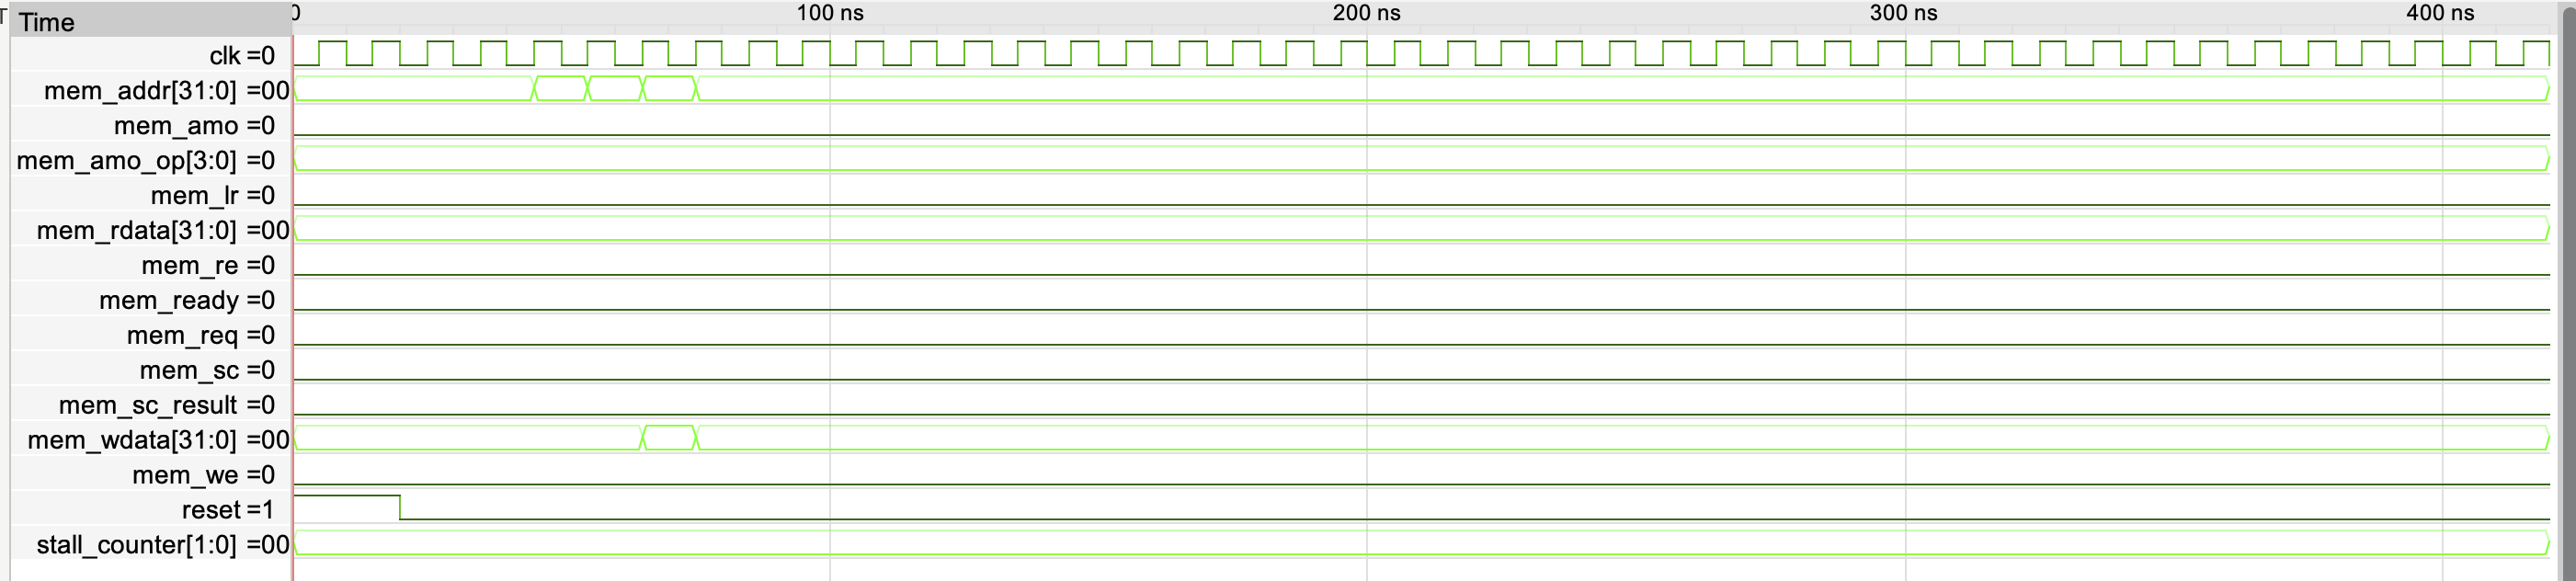
\includegraphics[width=0.92\textwidth]{design/test/risc_core.png}%
        }{%
            \fbox{\parbox[c][3.2cm][c]{0.88\textwidth}{\centering
                Chưa có ảnh \texttt{design/test/risc\_core.png}.}}
        }
        \vspace{0.3cm}
    \end{block}
    \vspace{0.1cm}
    \scriptsize
    \textbf{Phân tích Waveform:}
    \begin{itemize}
        \item Tín hiệu \texttt{PC} tăng tiến tuần tự +4 mỗi chu kỳ, nhảy đúng khi gặp lệnh \texttt{BEQ}/\texttt{JAL}.
        \item Các tín hiệu valid của pipeline (\texttt{if\_id\_valid}, \texttt{id\_ex\_valid}) bị xóa sạch tại thời điểm Flush.
        \item Tín hiệu \texttt{mem\_req} dựng lên khi core thực hiện \texttt{LW}/\texttt{SW}, \texttt{mem\_ready} phản hồi sau 1 chu kỳ.
    \end{itemize}
\end{frame}

% ==========================================
% TẦNG 4: KIỂM THỬ TOÀN HỆ THỐNG 8-CORE
% ==========================================
\subsection{Tầng 4: Kiểm Thử Toàn Hệ Thống}

% --- SLIDE: System Test Console Results ---
\begin{frame}[fragile]{Tầng 4: Kết Quả Kiểm Thử Hệ Thống 8-Core}
    Tích hợp toàn bộ 8 lõi CPU chạy song song, kết nối qua \textbf{Arbiter} và \textbf{Bus Controller} truy cập RAM dùng chung.
    \vspace{0.1cm}

    \begin{columns}[T]
        \begin{column}{0.42\textwidth}
            \textbf{Đánh giá hiệu năng:}
            \begin{itemize}
                \scriptsize
                \item 8 core cùng thực thi, ghi/đọc RAM dùng chung \textbf{không deadlock}.
                \item \texttt{grant} công bằng cho tất cả các nhân.
                \item \texttt{mem\_stall} tăng tuyến tính từ Core 0 $\rightarrow$ Core 7 $\Rightarrow$ đúng hành vi Round-Robin.
            \end{itemize}

            \begin{block}{Chỉ số xác thực}
                \scriptsize
                \begin{itemize}
                    \item \texttt{mem[0] == 42}: Dữ liệu ghi đúng.
                    \item \texttt{mem[1] == 99}: Marker hoàn thành.
                    \item 8/8 core: \texttt{grant > 0} và \texttt{retired > 0}.
                \end{itemize}
            \end{block}
        \end{column}

        \begin{column}{0.58\textwidth}
            \begin{block}{Kết quả Console (\texttt{system\_tb.v})}
                \fontsize{5pt}{6pt}\selectfont
                \begin{verbatim}
=========================================================
  BAT DAU MO PHONG HE THONG 8 LOI PIPELINE
=========================================================
  Kiem tra mem[0] (Ky vong: 42) = 42
    [PASS] Shared memory data dung.
  Kiem tra mem[1] addr 4 (Ky vong: 99) = 99
    [PASS] 8 core hoan thanh khong deadlock.

=========================================================
  PIPELINE / BUS EVIDENCE
=========================================================
  Core 0: grant=3 retired=163 mem_stall=13 flush=159
  Core 1: grant=3 retired=163 mem_stall=14 flush=159
  Core 2: grant=3 retired=163 mem_stall=15 flush=159
  Core 3: grant=3 retired=163 mem_stall=16 flush=159
  Core 4: grant=4 retired=161 mem_stall=17 flush=157
  Core 5: grant=4 retired=161 mem_stall=18 flush=157
  Core 6: grant=4 retired=161 mem_stall=19 flush=157
  Core 7: grant=4 retired=161 mem_stall=20 flush=157

  TONG KET: 10 PASSED, 0 FAILED
=========================================================
                \end{verbatim}
            \end{block}
        \end{column}
    \end{columns}
\end{frame}

% --- SLIDE: Waveform Hệ Thống 8-Core (Placeholder cho ảnh chụp) ---
\begin{frame}{Tầng 4: Waveform Mô Phỏng Hệ Thống 8-Core}
    \begin{block}{Giản đồ sóng toàn hệ thống (\texttt{system\_tb.vcd})}
        \centering
        \vspace{0.3cm}
        % === BẠN CHỤP WAVEFORM VÀ THAY TÊN FILE TẠI ĐÂY ===
        \IfFileExists{design/test/top_8core.png}{%
            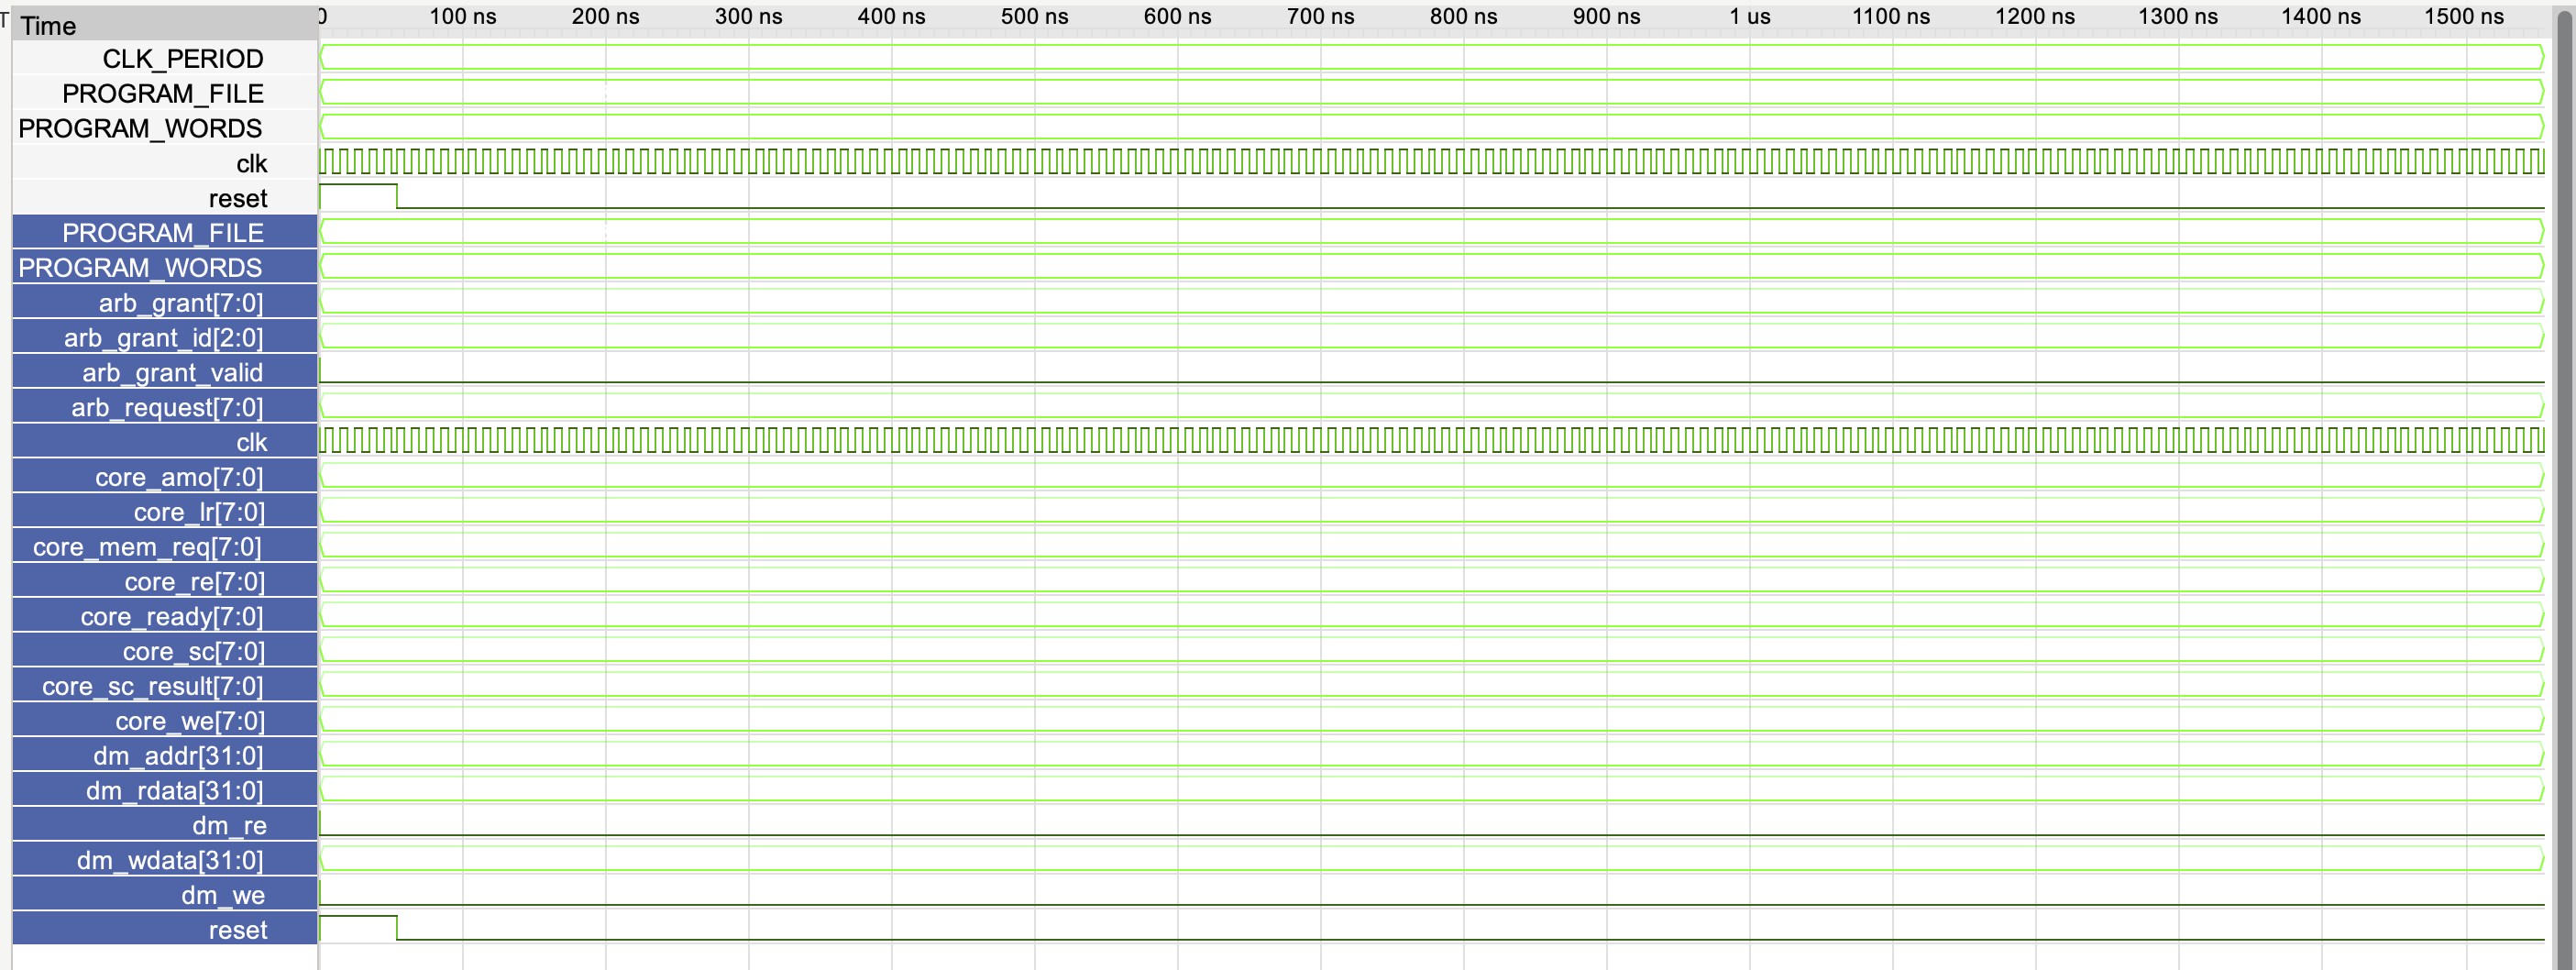
\includegraphics[width=0.92\textwidth]{design/test/top_8core.png}%
        }{%
            \fbox{\parbox[c][3.2cm][c]{0.88\textwidth}{\centering
                Chưa có ảnh \texttt{design/test/top\_8core.png}.}}
        }
        \vspace{0.3cm}
    \end{block}
    \vspace{0.1cm}
    \scriptsize
    \textbf{Phân tích Waveform:}
    \begin{itemize}
        \item Tín hiệu \texttt{grant[7:0]} của Arbiter phân phối quyền truy cập bus xoay vòng công bằng giữa 8 lõi.
        \item Các core chờ đợi (\texttt{mem\_stall}) khi chưa được cấp bus, tiếp tục xử lý Pipeline khi nhận \texttt{mem\_ready}.
        \item Không xảy ra tình trạng 2 core đồng thời giữ \texttt{grant = 1} (đảm bảo Mutual Exclusion).
    \end{itemize}
\end{frame}


\end{document}